\documentclass[a4paper, 12pt]{article}

\usepackage[left = 1cm,
            right = 1cm,
            top = 1cm,
            bottom = 1cm,
            footskip = 0cm]{geometry}
\usepackage{graphicx} % Required for inserting images
\usepackage{wrapfig}
\usepackage{listings}
\usepackage{xcolor}

\linespread{0.9}
\setlength{\parskip}{0pt}

\definecolor{codebackground}{rgb}{0.95,0.95,0.92} % Couleur de fond du code
\definecolor{codepurple}{rgb}{0.58, 0, 0.82}
\definecolor{codegreen}{rgb}{0, 0.6, 0}

\lstdefinestyle{mystyle}{
    language=C++,
    basicstyle=\scriptsize\ttfamily,
    frame=single,
    rulecolor=\color{black},
    backgroundcolor=\color{codebackground},
    commentstyle=\color{codegreen},
    keywordstyle=\color{blue},
    numberstyle=\tiny\color{codepurple},
    stringstyle=\color{red},
    lineskip={-1.5pt}
}

\lstset{style=mystyle}

\title{\textbf{Rapport pour le projet de INFOF202}}
\author{
    Ransy Lenny
    \and
    Lejeune Lucas
    }
\date{Janvier 2024}
\renewcommand*\contentsname{Table des matières}

\begin{document}
\setlength{\parindent}{0em}

\maketitle

Ce rapport vise a documenter le projet "Frogger" que nous avons réaliser. Nous traiterons les tâches que nous avons réalisées et comment nous les avons réalisées. Pour cela, nous parlerons des classes que nous avons codées pour faire ce projet, comment elles sont réparties dans le code et comment elles intéragissent entre elles. Nous justifierons aussi comment nous avons utilisé le modèle de conception MVC dans la partie jeu.

\section{Résumé des tâches réalisées et fonctionnement du jeu}
% Résumer comment le jeu marche et listes les tâches réalisées
Nous avons réalisé les tâches principales et toutes les tâches additionnelles, sauf la tâches de l'éditeur de niveau. 
Ouvrons le jeu et voyons ce qui se passe. 
% Parler du fonctionnement du jeu quand tout sera fini

\section{Structure des fichiers: Utilisation du MVC}
% Parler de l'orga des fichiers

La structure des fichiers peut se diviser en plusieurs parties: les fichiers du jeu, ceux des menus, les mains et les images du jeu. \\

\begin{wrapfigure}{r}{3cm}
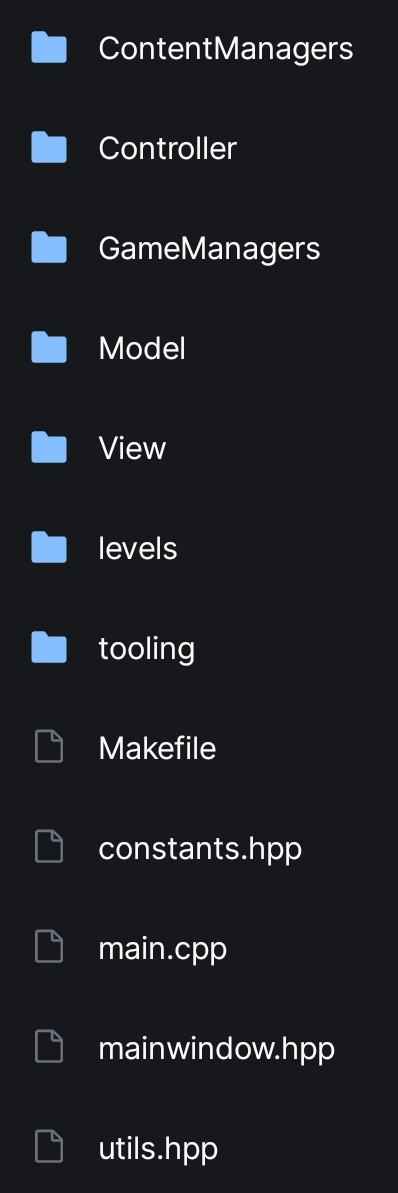
\includegraphics[width=3cm]{Images/folders.jpg}
\end{wrapfigure}

Le dossier \texttt{ContentManagers} contient tout les fichiers de code en rapport avec la gestion des menus du jeu.\\

Les dossiers \texttt{Controller}, \texttt{Model} et \texttt{View} contiennent le code parmettant de faire tourner le jeu (la partie plateau, qui ne compte pas le menu).
Cette disposition met en évidence l'utilisation du MVC. Prenons la gestion de la grenouille comme exemple. 
Les fichiers gérant les contrôles de celle-ci se trouvent dans le dossier \texttt{Controller}, ceux qui gèrent ses propriétés dans le plateau se trouvent dans \texttt{Model} et enfin, ceux qui gèrent son affichage se trouvent dans \texttt{View}. Tout le code de ces fichiers est utilisé dans les fichiers de \texttt{GameManagers} pour avoir un jeu fonctionnel.\\

Le dossier \texttt{levels} contient les données des niveaux sauvegardés en fichiers \texttt{.csv}, et les scores obtenus sur ceux-ci. Plus de détails seront donnés dans les chapitres concernés. \\

Le dossier \texttt{tooling} contient tout les outils construits grâce aux outils venant la librairie FLTK qui sont surtout utilisés dans la partie \texttt{View} et \texttt{ContentManagers}. \\

Le fichiers \texttt{constants.hpp} contient toutes les constantes utilisées dans le projet, comme par exemple la taille des bouttons dans le menu. \\

Enfin, les fichiers \texttt{main.cpp} et \texttt{mainwindow.hpp} s'occupent d'assembler toutes les classes et fonctions ensemble, pour obtenir l'application Frogger au complet. 

\section{Réalisation de la base du jeu (Tâches de base)}
% On parle du tout début juste avec les roadlanes
Bien sûr, pour cette tâche, la première chose à faite a été de faire un support pour utiliser fltk. C'est là que les fichiers \texttt{main.cpp} et \texttt{MainWindow.hpp} rentrent en jeu.

\subsection{Modèle}

Il nous faut maintenant un modèle fonctionnel. Le but est de d'abord faire un plateau de jeu. \\

Les rangées sont des objets de classe \texttt{Lane}, classe qui est définie dans le fichier \texttt{lanes.hpp}.

\begin{lstlisting}
class Lane {
    private:
        const unsigned int id_num;
    public:
        Lane(const unsigned int id_num);
        unsigned int getId() const;
        virtual void dive_update() {}
        virtual ~Lane() {}
};  
\end{lstlisting}

La classe \texttt{BoardModel} contient alors un vecteur de pointeurs vers des objets \texttt{Lane}.

\begin{lstlisting}
class BoardModel {
private:
    std::shared_ptr<FinishLane> the_finish_lane;
    std::vector<std::shared_ptr<Lane>> lanes {};
    unsigned time = 0;
public:
    BoardModel(std::vector<std::shared_ptr<Lane>> lanes);
    void update_turtles(std::shared_ptr<Lane> lane);
    void update(); // moves the objects on the board
    bool gameWon();
    bool isOutOfBoard(Frog& frog);
    bool frogOnLily(Frog& frog);
    void addLane(std::shared_ptr<Lane> lane);
    std::vector<std::shared_ptr<Lane>> getLanes();
    bool any_collision(Frog& frog);
    void handle_collision(Frog& frog);
    ~BoardModel() {}
    unsigned getTime() const  { return time; }
};
\end{lstlisting}

Pour avoir différents types de rangées, il suffit alors de définir ces types grâce à de l'héritage sur la classe \texttt{Lane}. Nous définissons alors dans le fichier \texttt{lane.hpp} les classes \texttt{FinnishLane} (nous en parlons dans le chapitre \ref{lilies}), \texttt{SafeLane} et \texttt{RoadLane}. \\

\begin{lstlisting}
class SafeLane: public Lane {
    public:
        SafeLane(const unsigned int id);
        ~SafeLane() {}
};
\end{lstlisting}

\begin{lstlisting}
class MovingObjectLane: public Lane {
    protected:
        std::vector<std::shared_ptr<MovingObject>> mv;
        int lane_speed;
    public:
        MovingObjectLane(const unsigned int id, int lane_speed=0);
        bool frog_collide(Frog& frog);
        std::vector<std::shared_ptr<MovingObject>> getMovingObjects();
        virtual void handle_after_collision(Frog& frog) = 0;
        virtual bool waterLane() const = 0 ;
        virtual ~MovingObjectLane() {}
};
\end{lstlisting}

\begin{lstlisting}
class RoadLane: public MovingObjectLane {
    public:
        RoadLane(const unsigned int id_num
                , const unsigned int& car_by_pack
                , const unsigned int& space_between_cars
                , const unsigned& space_between_packs
                , const int& first_car_placement
                , const unsigned int& size_car
                , const int& speed=1);
        bool waterLane() const override { return 0; }
        void handle_after_collision(Frog& frog) override;
        std::vector<std::shared_ptr<Car>> getCars() const;
         ~RoadLane() {}
};
\end{lstlisting}

Nous voulons d'abord définir ce qu'est une voiture, ceci se passe dans le fichier \texttt{movingobjects.hpp}. \\

\begin{lstlisting}
    class MovingObject {
        protected:
          const int speed;
          int x;
          const unsigned int size;
          const unsigned int lane_id;
        public:
          MovingObject(const int speed, int x, const unsigned int size, const unsigned lane_id);
          void move();
          unsigned getSize() const;
          unsigned getId() const;
          // returns the x coordinate of the center of the object
          int getCenterX() const;
          std::tuple<int, int> getBoundaries() const;
          int getX() const;
          // returns true if this element collides with the frog
          virtual bool collide(Frog& frog) = 0;
          int getSpeed() const;
      
          // Methods regarding diving turtles
          virtual void dive() {}
          virtual void undive() {}
          virtual bool isDiving() const;
          virtual ~MovingObject() {}
      };
\end{lstlisting}

\begin{lstlisting}
    class Car: public MovingObject {
    public:
        Car(int speed, unsigned int head, const unsigned int size, const unsigned lane_id);
        bool collide(Frog& frog) final override;
        ~Car() {}
    };
\end{lstlisting}

Toutes les classes et méthodes sont après assemblées dans la classe \texttt{BaordModel} pour faire un plateau fonctionnel. \\

Parlons maintenant de la grenouille. Elle sera définie par un objet de classe \texttt{Frog}, classe qui est définie dans le fichier \texttt{frog.hpp}.

\begin{lstlisting}
class Frog {
    private:
        // Frog Position and Direction (important for display)
        unsigned int lane_number;
        int x;
        FrogDirection direction = FrogDirection::North;
        int lives;
        std::shared_ptr<Score> score;
    public:
        Frog(unsigned int lane_number, int x, std::shared_ptr<Score> score);

        // Standard getters
        unsigned int getLane() const ;
        int getX() const;
        int getLives() const;
        FrogDirection getDirection() const;

        // Methods in charge of moving the frog (interacting with the controller)
        void goUp();
        void goDown();
        void goLeft();
        void goRight();

        // Moves the frog in a given direction (helpful when frog is sitting on logs)
        void go(int speed);
        // Returns false only if the frog is outside
        bool inBoard();

        // Methods in charge of life and death of the frog
        void resetPos();
        bool alive();
        void kill();
        void inWaterLilies();

        ~Frog(){}
};
\end{lstlisting}

\subsection{Controlleur}

Les contrôles de la grenouille se passent dans la classe \texttt{Controller} qui se trouve quand le fichier \texttt{controller.hpp} qui est contenu dans le dossier \texttt{Controller}.
La classe \texttt{Frog} possède déjà des méthodes permettant de changer sa position sur le plateau, il faut alors juste les utiliser quand nous appuyons sur une touche. La méthode \texttt{processKey} sert à gérer ces actions. Les contrôles se font avec les touches zqsd comme pour beaucoup de jeux. 

\begin{lstlisting}
    class Controller {
    private:
        std::shared_ptr<Frog> f;
        std::map<char, bool> is_pressed;
        unsigned int count = 0;
    public:
        Controller(std::shared_ptr<Frog> f);
        void decrement();
        void processKey(char& c);
        void updatePressedKeys(const char&& c);
        void resetPressedKeys();
        ~Controller() {}
};
\end{lstlisting}

\subsection{Vue}

Tout ce dont nous allons parler dans ce sous-chapitre se passe dans le dossier \texttt{View}. Pour résumer, pour presque chaque classe de la partie modèle, il y a une classe de la partie vue qui s'occupe de l'affichage de ce modèle.
L'intérêt de ces classes est de pouvoir utiliser la méthode \texttt{draw} pour afficher l'objet sur la plateau. \\

\underline{Dans movingobjectview.hpp:} \hspace{0.5cm}

\begin{lstlisting}
    class MovingObjectView {
    protected:
        std::shared_ptr<MovingObject> mv;
        std::unique_ptr<RectangleDrawer> object_drawer;
    public:
        MovingObjectView(std::shared_ptr<MovingObject> mv);
        virtual void draw();
        std::shared_ptr<MovingObject> getMovin();
        virtual ~MovingObjectView() {}
};
\end{lstlisting}

\begin{lstlisting}
class CarView: public MovingObjectView {
    public:
        CarView(std::shared_ptr<Car> c);
        ~CarView() {}
};
\end{lstlisting}

\underline{Dans laneview.hpp:} \hspace{0.5cm}

\begin{lstlisting}
    /// An abstract class that helps model a lane
    class Lane {
        private:
            const unsigned int id_num;
        public:
            Lane(const unsigned int id_num);
            unsigned int getId() const;
            virtual void dive_update() {}
            virtual ~Lane() {}
    };
\end{lstlisting}

\begin{lstlisting}
    class FinishLane: public Lane {
        private:
            std::vector<std::shared_ptr<WaterLilies>> lilies;
        public:
            FinishLane(const unsigned int id);
            std::vector<std::shared_ptr<WaterLilies>> getLilies();
            ~FinishLane() {}
    };
\end{lstlisting}

\begin{lstlisting}
    class SafeLane: public Lane {
        public:
            SafeLane(const unsigned int id);
            ~SafeLane() {}
    };
\end{lstlisting}

\begin{lstlisting}
    class MovingObjectLane: public Lane {
        protected:
            std::vector<std::shared_ptr<MovingObject>> mv;
            int lane_speed;
        public:
            MovingObjectLane(const unsigned int id, int lane_speed=0);
            bool frog_collide(Frog& frog);
            std::vector<std::shared_ptr<MovingObject>> getMovingObjects();
            virtual void handle_after_collision(Frog& frog) = 0;
            virtual bool waterLane() const = 0 ;
            virtual ~MovingObjectLane() {}
    };   
\end{lstlisting}

\begin{lstlisting}
class RoadLane: public MovingObjectLane {
    public:
        RoadLane(const unsigned int id_num
                , const unsigned int& car_by_pack
                , const unsigned int& space_between_cars
                , const unsigned& space_between_packs
                , const int& first_car_placement
                , const unsigned int& size_car
                , const int& speed=1);
        bool waterLane() const override { return 0; }
        void handle_after_collision(Frog& frog) override;
        std::vector<std::shared_ptr<Car>> getCars() const;
        ~RoadLane() {}
};
\end{lstlisting}

Nous parlerons de l'affichage de la grenouille dans les chapitres \ref{lives} et \ref{frogview} \\

\underline{Dans boardview.hpp:} \hspace{0.5cm}

\begin{lstlisting}
    class BoardView {
        private:
          std::vector<std::shared_ptr<LaneView>> lanes;
          std::shared_ptr<BoardModel> b;
        public:
          BoardView(std::vector<std::shared_ptr<LaneView>> lanes,
                    std::shared_ptr<BoardModel> b);
          void draw();
          std::vector<std::shared_ptr<LaneView>> getLaneList();
          ~BoardView() {}
      };
\end{lstlisting}


\subsection{Assemblage pour faire un jeu fonctionnel}

Il nous faut maintenant assembler le tout pour faire un plateau fonctionnel. Ceci se fait dans le dossier \texttt{GameManagers}, et plus particulièrement dans le fichier \texttt{gameloop.hpp}. Dans celui-ci se trouve la classe \texttt{GameLoop} prennant tout ce que nous avons défini (et d'autres éléments dont nous parlerons plus tard) en instance. Le plateau s'initialise alors avec le constructeur, et s'anime en exécutant à chaque frame la méthode \texttt{update}. Nous verrons plus tard où cette méthode est exécutée.

\begin{lstlisting}
class GameLoop {
    private:
        std::shared_ptr<BoardModel> bm;
        std::shared_ptr<BoardView> bv;
        std::shared_ptr<FrogView> fv;
        std::shared_ptr<Frog> frog;
        std::shared_ptr<Score> score;
        std::shared_ptr<ScoreView> sv;
        std::shared_ptr<Controller> c;
        std::unique_ptr<ScoreSaver> ssv;
        std::shared_ptr<Score> best_score;
        std::unique_ptr<ScoreView> bs_show;
    public:
        GameLoop(unsigned int lvl);
        void update();
        std::shared_ptr<BoardModel> getModel();
        std::shared_ptr<BoardView> getView();
        std::shared_ptr<FrogView> getFrog();
        ~GameLoop() {}
};
\end{lstlisting}

\section{Réalisation des tâches additionnelles}
Maintenant que les tâches principales sont réalisées et que nous avons une bonne base, nous pouvons implémenter les fonctionnalités supplémentaires. 

\subsection{Rangées d'eau, buches et tortues} \label{turtle_class}

\underline{\textbf{Modèle:}} 
Dans le fichier \texttt{movingobjects.hpp}, nous implémentons les tortues et les buches. Les collisions ne seront pas gérée de la même manière que pour les voitures, donc nous faisons un override. Nous parlerons plus en détail des méthodes de la classe \texttt{Turtle} dans le chapitre \ref{diving_turtles}. \\

\begin{lstlisting}
class Turtle: public MovingObject {
    private:
        bool diving;
    public:
        Turtle(int speed, const unsigned int head, const unsigned int size
                , const unsigned lane_id);
        void dive() final override;
        void undive() final override;
        bool isDiving() const final override;
        bool collide(Frog& frog) final override;
        ~Turtle() {}
};
\end{lstlisting}

\begin{lstlisting}
class Log: public MovingObject {
    public:
        Log(int speed, unsigned int head, const unsigned int size,
            const unsigned lane_id);
        bool collide(Frog& frog) final override;
        ~Log() {}
};
\end{lstlisting} \hspace{0.5cm}

Dans le fichier \texttt{lane.hpp}, nous implémentons deux nouvelles classes héritantes de \texttt{MovingObjectLane}. 
Nous parlerons aussi plus tard des méthodes de la classe \texttt{TurtleLane}. \\

\begin{lstlisting}
class LogLane: public MovingObjectLane {
    public:
        LogLane(const unsigned int id_num, const unsigned int& log_by_pack,
                const unsigned int& space_between_logs,
                const unsigned& space_between_packs,
                const int& first_log_placement,
                const unsigned int& size_log, const int& speed=0);
        bool waterLane() const override { return 1; }
        void handle_after_collision(Frog& frog) override;
        std::vector<std::shared_ptr<Log>> getLogs() const;
        ~LogLane() {}
};
\end{lstlisting}

\begin{lstlisting}
class TurtleLane: public MovingObjectLane {
    unsigned int turtle_by_pack;
    unsigned int diving_pack_id;
    bool is_diving = true;
    unsigned int diving_time;   // In frames
    unsigned int undiving_time;
    unsigned int diving_count = 0;
    public:
        TurtleLane(const unsigned int id_num
                   , const unsigned int& turtle_by_pack
                   , const unsigned int& space_between_turtles
                   , const unsigned& space_between_packs
                   , const int& first_turtle_placement
                   , const unsigned int& size_turtle
                   , const int& speed=1
                   , const unsigned int diving_pack_id = 0
                   , const unsigned int diving_time = 180
                   , const unsigned int undiving_time = 180);
        std::vector<std::shared_ptr<Turtle>> getTurtles() const;
        void handle_after_collision(Frog& frog) override;
        bool waterLane() const override { return 1; }
        void pack_dive();
        void pack_undive();
        void dive_update() final override;
        ~TurtleLane() {}
};
\end{lstlisting} \hspace{0.5cm}

% Parler des mouvements de la grenouille quand sur ces objets

\underline{\textbf{Vue:}} \\
Les implémentations gérant la vue de ces deux nouvelles rangées est similaire que pour celle des rangées de voitures. \\
\begin{lstlisting}
class LogView: public MovingObjectView {
    public:
        LogView(std::shared_ptr<Log> l);
        ~LogView() {}
};
\end{lstlisting}

\begin{lstlisting}
class TurtleView: public MovingObjectView {
    public:
        TurtleView(std::shared_ptr<Turtle> t);
        void draw() final override;
        ~TurtleView() {}
};
\end{lstlisting}

\subsection{Nénuphars} \label{lilies}

Dans le fichier \texttt{Model/waterlilies.hpp}, nous définissons une nouvelle classe \texttt{WaterLilies} qui va représenter les nénuphars. \\

\begin{lstlisting}
class WaterLilies {
    private:
        int x;
        bool visited=false;
    public:
        WaterLilies(int x);
        int getX();
        bool collide(Frog& frog);
        bool hasBeenVisited();
        void visit();
        ~WaterLilies() {}
};
\end{lstlisting} \hspace{0.5cm}

Nous pouvons maintenant parler de l'implémentation de la classe \texttt{FinishLane}. \\

\begin{lstlisting}
class FinishLane: public Lane {
    private:
        std::vector<std::shared_ptr<WaterLilies>> lilies;
    public:
        FinishLane(const unsigned int id);
        std::vector<std::shared_ptr<WaterLilies>> getLilies();
        ~FinishLane() {}
};
\end{lstlisting} \hspace{0.5cm}

\subsection{Vies de la grenouille} \label{lives}

Les vies de la grenouille sont représentées par l'instance \texttt{lives} de la classe \texttt{Frog}. A chaque exécution de 
\texttt{GameLoop::update()}, on regarde si la grenouille respecte une des conditions pour perdre une vie. Si oui, alors on décrémente \texttt{lives} avec la méthode \texttt{kill()}. Si \texttt{lives} est à 0, alors on affiche un écran de défaite de la même manière que nous l'avons fait avec la victoire (avec le fichier \texttt{imgs/lose.jpeg}. \\

La classe \texttt{FrogView} s'occupe de dessiner tout ce qui est relié à la grenouille. Nous parlons ici seulement des vies, le reste sera abordé dans le chapitre \ref{frogview}. La méthode \texttt{showLives()} est alors appelée dans la méthode \texttt{draw()}. \\

\begin{lstlisting}
class FrogView {    
    std::shared_ptr<Frog> frog;
    JPEGDrawer current_image{paths::frog_north_jpeg, frog->getX(),
                                static_cast<int>(frog->getLane()), HEIGHT, WIDTH};
public:
    FrogView(std::shared_ptr<Frog> f);
    void showLives();
    void draw();
};
\end{lstlisting}

\subsection{Tortues plongeantes} \label{diving_turtles}

Dans le modèle, une tortue plonge si son instance \texttt{diving} est à \texttt{True} (voir \ref{turtle_class}). Ce statut change surtout le comportement des collisions avec les tortues dans le modèle. Nous ordonnons à la tortue de plonger avec les méthodes \texttt{dive()} et \texttt{undive()}. Ces ordres sont alors données dans la classe \texttt{TurtleLane} (voir \ref{turtle_class}). Comme dans le jeu orginal, nous faisons plonger les tortues par paquets. Nous pouvons choisir les intervalles de temps entre la plongée et la remontée des tortues d'un paquet d'une rangée dans les paramêtres du constructeur de la classe. Nous pouvons aussi choisir quel paquet va plonger dans les paramêtres. La méthode \texttt{dive\textunderscore update()} va alors se charger de faire plonger et remonter les tortues en boucle avec les paramêtres choisis. Cette méthode est exécutée à chaque frame dans la méthode \texttt{GameLoop::update()}. \\

Nous changons forcément commment est affichée la tortue quand elle plonge. Pour cela, nous faisons en sorte que la méthode \texttt{TurtleView::draw()} ne marche que quand la tortue est à la surface.

\subsection{Directions de la grenouille} \label{frogview}
Les directions sont gérées avec l'enum class suivant:
\begin{lstlisting}
enum class FrogDirection {
    North, South, East, West
};
\end{lstlisting}
\subsection{Score}
\begin{lstlisting}
class Score {
    private:
        unsigned the_score = 0;
        int max_lane = 0;
    public:
        Score() = default;
        Score(unsigned score): the_score(score) {}

        void reachedWaterlily();
        void update(int new_lane_id);
        unsigned getScore() const;
        void resetBestLane();

        friend bool operator<(Score const& s1, Score const& s2);
        friend bool operator>(Score const& s1, Score const& s2);
        friend bool operator==(Score const& s1, Score const& s2);
        ~Score() = default;
};
\end{lstlisting}
\subsection{Meilleur score}
Le meilleur score et l'interaction avec les fichiers est gérée par la classe ScoreSaver
\begin{lstlisting}
class ScoreSaver {
    private:
        unsigned lvl;
        const std::string file_name { paths::scores };
        std::map<unsigned, unsigned> scores;
    public:
        ScoreSaver(unsigned level): lvl(level) {}
        void writeToFile();
        void getFromFile();

        Score getHighScore();
        void setNewScore(Score const& score);
        void resetHighScore();
        void setLevel(unsigned& level);
        ~ScoreSaver() {}
};
\end{lstlisting}
\subsection{Gestion des menus et écran d'accueil}
La majorité des fichiers chargés de la gestion de smenus se trouvent dans ContentManagers.
\begin{lstlisting}
class WindowContents;

class ContentManager {
    private:
        std::unique_ptr<WindowContents> contents;
        std::unique_ptr<GameLoop> gl;
    public:
        ContentManager(std::unique_ptr<WindowContents> first_contents):
            contents(std::move(first_contents)), gl(nullptr) {}

        void changeContents(std::unique_ptr<WindowContents> new_contents);

        void manageButtonPush(int x, int y);

        void contentManageAction(actions& action);

        void startGame(std::unique_ptr<GameLoop> g);
        void show();

        static void updateWithAction(std::shared_ptr<ContentManager> cm, actions& action);

        ~ContentManager() { }
};

class WindowContents {
   protected:
        std::weak_ptr<ContentManager> cm; // Observer
    public:
        WindowContents(std::shared_ptr<ContentManager> cm): cm(cm) {}
        WindowContents(std::weak_ptr<ContentManager> cm): cm(cm) {}
        virtual void draw() = 0;
        virtual void manageButtonPush(int x, int y) = 0;
        virtual void manageAction(actions& action) = 0;
        std::weak_ptr<ContentManager> getCM() {
            return cm;
        }

        virtual ~WindowContents() {}
};
\end{lstlisting}
En clair, ces classes fonctionnent de la manière suivante:
Ce qui est affiché dans la fenêtre hérite de WindowContents, ainsi, nos menus, et la sélection de niveau héritera de WindowContents, ContentManager est la classe se chargeant d'alterner les différents contenus que l'on affiche à l'écran,
par exemple, si je décide d'appuyer sur le bouton pour aller au menu de sélection de niveau, le menu de sélection de niveau et le menu de base sont tous les deux des WindowContents, et ce qui permet de changer entre les deux est l'instance de ContentManager.

L'écran d'accueil est représenté par la classe suivante
\begin{lstlisting}
class WelcomeScreen: public WindowContents {
    private:
        ActionButton start_game_button;
        ActionButton go_to_levels;
        Text welcome;
   public:
        WelcomeScreen(std::shared_ptr<ContentManager> cm): WindowContents(cm) {}
        void manageButtonPush(int x, int y) override;
        void manageAction(actions& action) override;
        void draw() override;
        ~WelcomeScreen() {}

};
\end{lstlisting}
\subsection{Niveaux et sélection de niveau}
\begin{lstlisting}
class LevelSelect: public WindowContents {
    public:
        LevelSelect(std::shared_ptr<ContentManager> cm): WindowContents(cm) {
            ss.getFromFile();
            best_score_show.setString("Highest Score: " + std::to_string(ss.getHighScore().getScore()));
        }
        LevelSelect(std::weak_ptr<ContentManager> cm): WindowContents(cm) {
            ss.getFromFile();
            best_score_show.setString("Highest Score: " + std::to_string(ss.getHighScore().getScore()));
        }
        void draw() override;
        void manageButtonPush(int x, int y) override;
        unsigned getLevel();
        void manageAction(actions& action) override;
        ~LevelSelect() {}

};
\end{lstlisting}

\end{document}
